\pagestyle{fancy}
\chapter{\heiti Installing Software}
\setmainfont{Times New Roman}
There is an u-disk in the accessories. And user can find the “ASG\_install” folder, that contains all the files to install the sequence editing PC software. 
%在随机箱附件的U盘中含有我司为用户提供的“ASG\_install”文件夹,里面包含安装方波序列编辑软件所需的全部文件。

\section{\heiti Installing python interpreter}
User can download the python 2.7 interpreter from http://www.python.org/ ( 32 bit version is recommended ), or user can run the installer named “Python-2.7.11.msi” in “ASG\_install” folder. When choosing the installing components, please check all,  then click “Next” to finish the installation procedure. The computer will install the python interpreter to “C:\textbackslash Python27 by default. After finishing installing the interpreter, click “begin” → “run”, then input “cmd” to enter the textbox to enter the command window. Fig 3.1 will show up after inputting “Python”, that represents the python interpreter has been installed. If get “Python is not internal or external command, nor a runnable program or batch file”, please restart your computer first, and then enter the command window. If you obtain the same result after inputting “Python”, right click “Computer”→, and then find the “Path”, add “;C:\textbackslash python (location of python interpreter)”. If still fail, please contact with us (sale@qpdtek.com).
%用户可到Python官网(http://www.python.org/)下载Python 2.7版本的解释器(推荐下载32位版本),也可运行我司提供的“ASG\_install”文件夹下“Python-2.7.11.msi”安装程序,在选择安装组件时,务必勾选所有组件,然后点击“Next”即可完成安装,计算机默认会将Python解释器安装到C:\textbackslash Python27 目录下。安装完成后,点击任务栏“开始”→“运行”,在弹出窗口中输入“cmd”,即可进入命令窗口。输入“Python” 后,若出现如图3.1 所示情况,则代表Python 解释器安装成功;若得到“Python不是内部或外部命令,也不是可运行的程序或批处理文件”,请先重启计算机,再进入命令窗口,输入“Python”后,若仍得到“Python不是内部或外部命令,也不是可运行的程序或批处理文件”,请右键“计算机” → “属性” →“ 系统高级设置” →“ 高级” → “环境变量”,然后在系统变量中找到Path,编辑此变量在后面追加“;C:\textbackslash python (python 安装位置)”。如果仍未安装成功,请联系合肥量子精密仪器有限公司(sale@qpdtek.com)。

%\begin{figure}[ht]
%\centering
%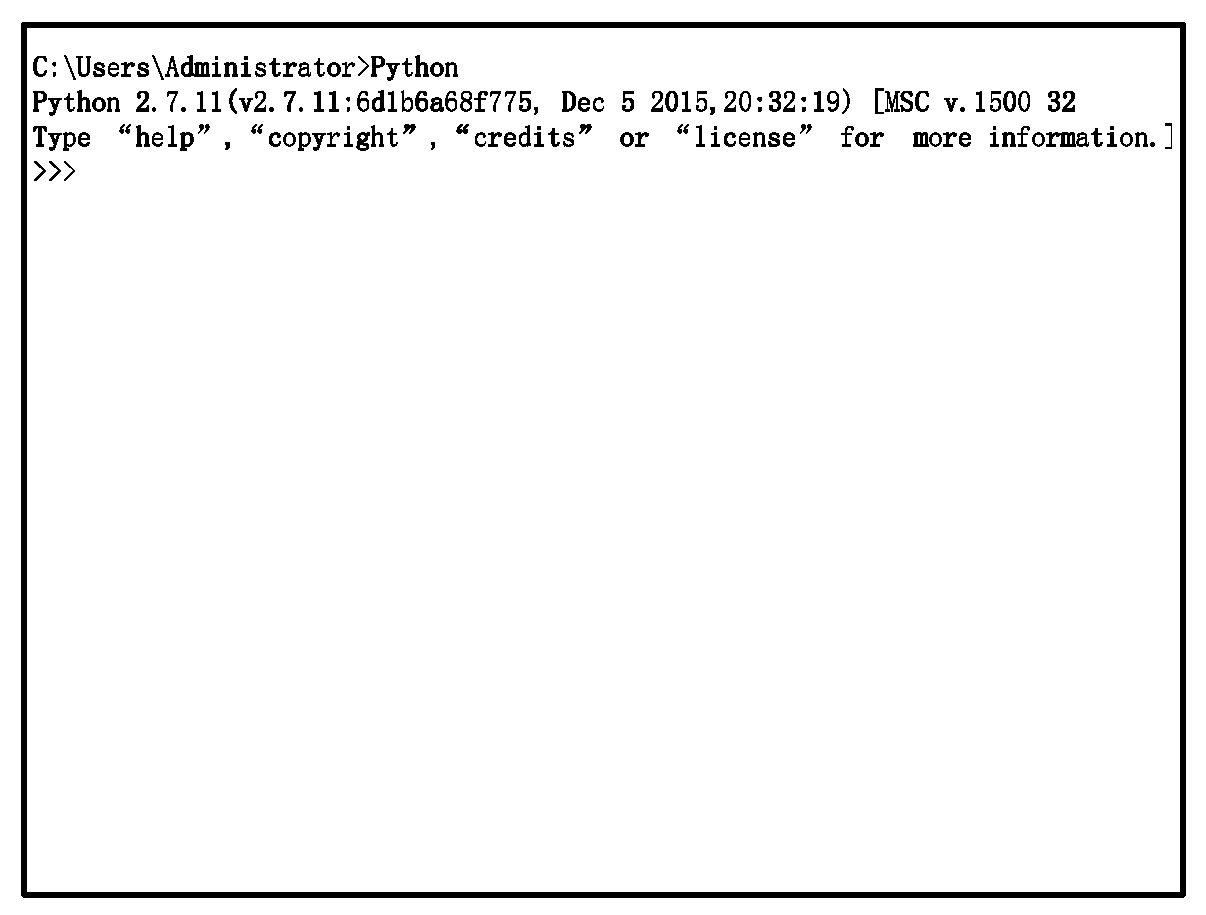
\includegraphics[width=10cm]{fig3_1}
%\caption{Python 安装勾选组件}
%\end{figure}
\begin{figure}[ht]
\centering
%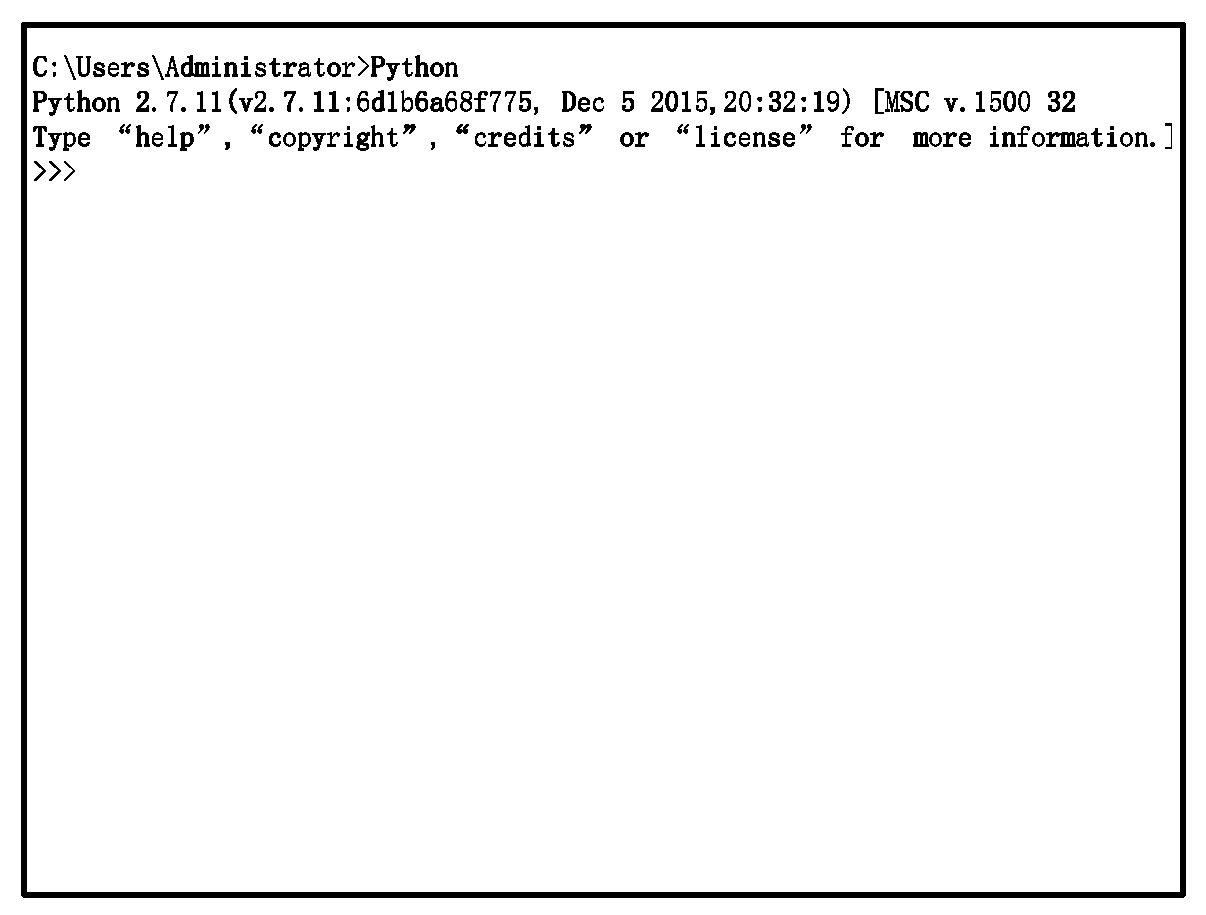
\includegraphics[width=9.6cm,height=7cm]{fig3_1}
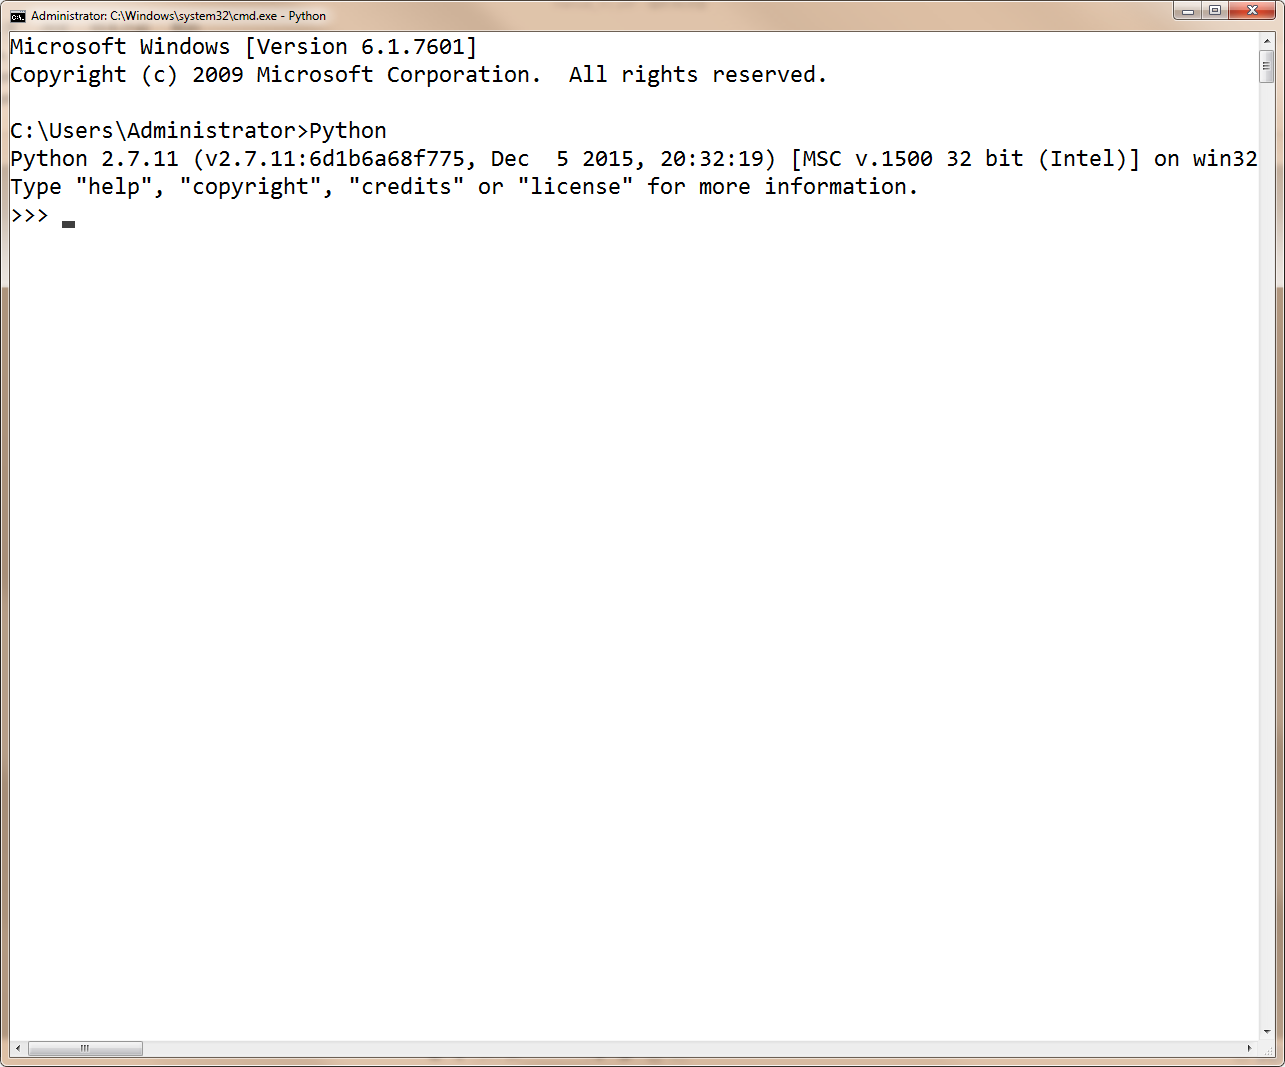
\includegraphics[height=7.5cm]{fig3_1_0}
\caption{The python interpreter has been installed successfully}
\end{figure}

\newpage
\section{\heiti Installing packages}
We offer all the python packages such as wxpython, matplotlib, numpy and six, to make the software runnable. Installing these packages can perform as below.
%我司会为用户提供运行软件所需的所有第三方Python库的安装文件,包括wxpython、matplotlib(包括dateutil文件与pyparsing文件)、numpy、six等。下面依次讲解如何安装这4个第三方库。
\vspace{0.3cm}

\noindent$\vcenter{\hbox{\huge$\bullet$}}$\quad\fontsize{12pt}{\baselineskip}\textbf{\heiti{Installing wxpython :}}

Please enter the “wxpython” folder in the “ASG\_install” folder, then double click the installation program and click “Next” will install the package. 
%进入我司为用户提供的ASG\_install文件夹下的wxpython文件夹,双击其中的exe安装程序,点击“Next”即可安装wxpython库。
\vspace{0.3cm}

%\newpage
\noindent$\vcenter{\hbox{\huge$\bullet$}}$\quad\fontsize{12pt}{\baselineskip}\textbf{\heiti{Instaling matplotlib :} }

Please enter the “matplotlib” folder in the “ASG\_install” folder, then double click the installation program and click "Next” will install the package. And then, user need to install “dateutil” and “pyparsing” .
%进入我司为用户提供的ASG\_install文件夹下的matplotlib文件夹,双击其中的exe安装程序,点击“Next”即可安装matplotlib库。安装matplotlib库后还需要安装dateutil与pyparsing两个文件。
\vspace{0.3cm}

\noindent$\vcenter{\hbox{\huge$\bullet$}}$\quad\fontsize{12pt}{\baselineskip}\textbf{\heiti{Installing dateutil :} }

Enter the command window, then use “cd” command to switch the current directory as the lacation that you deposit the “matplotlib” folder. For example, if user put the “ASG\_install” folder in the root director of E disk, please input “E:” → “cd ASG\_install” → “cd matplotlib” , and then input “pip install python\_dateutil-2.6.0-py2.py3-none-any.whl” to install dateutil file. The whole installation procedure will be shown in Fig 3.2 .
%进入Windows命令窗口(点击任务栏“开始”→“运行”,在弹出窗口中输入“cmd”后点击“确定”),然后使用“cd”命令将当前目录切换到您存放我司提供的matplotlib文件夹所在位置。如用户将ASG\_install文件夹放在E 盘的主目录下,在命令窗口中依次输入“E:” → “cd ASG\_install” → “cd matplotlib”,即可将当前目录切换到存放matplotlib文件夹的位置。然后通过“pip install python\_dateutil-2.6.0-py2.py3-none-any.whl” 命令安装dateutil 文件。完整过程为如图3.2,依次输入命令即可安装dateutil 文件。
\begin{figure}[ht]
\centering
%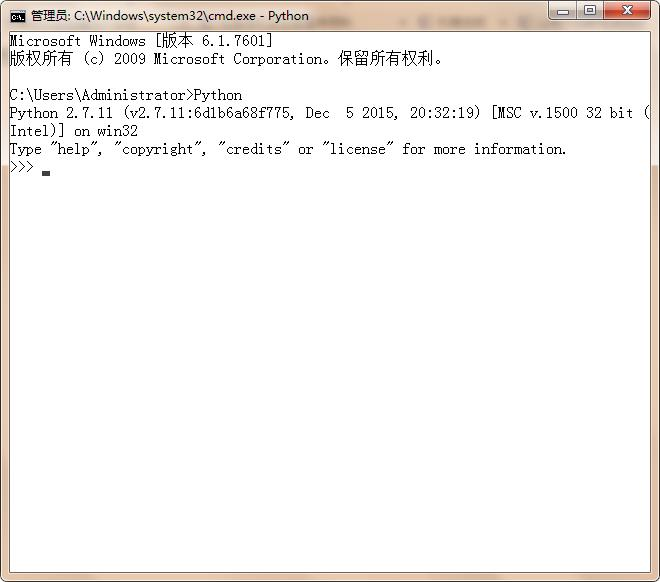
\includegraphics[width=9.6cm,height=7cm]{fig3_2}
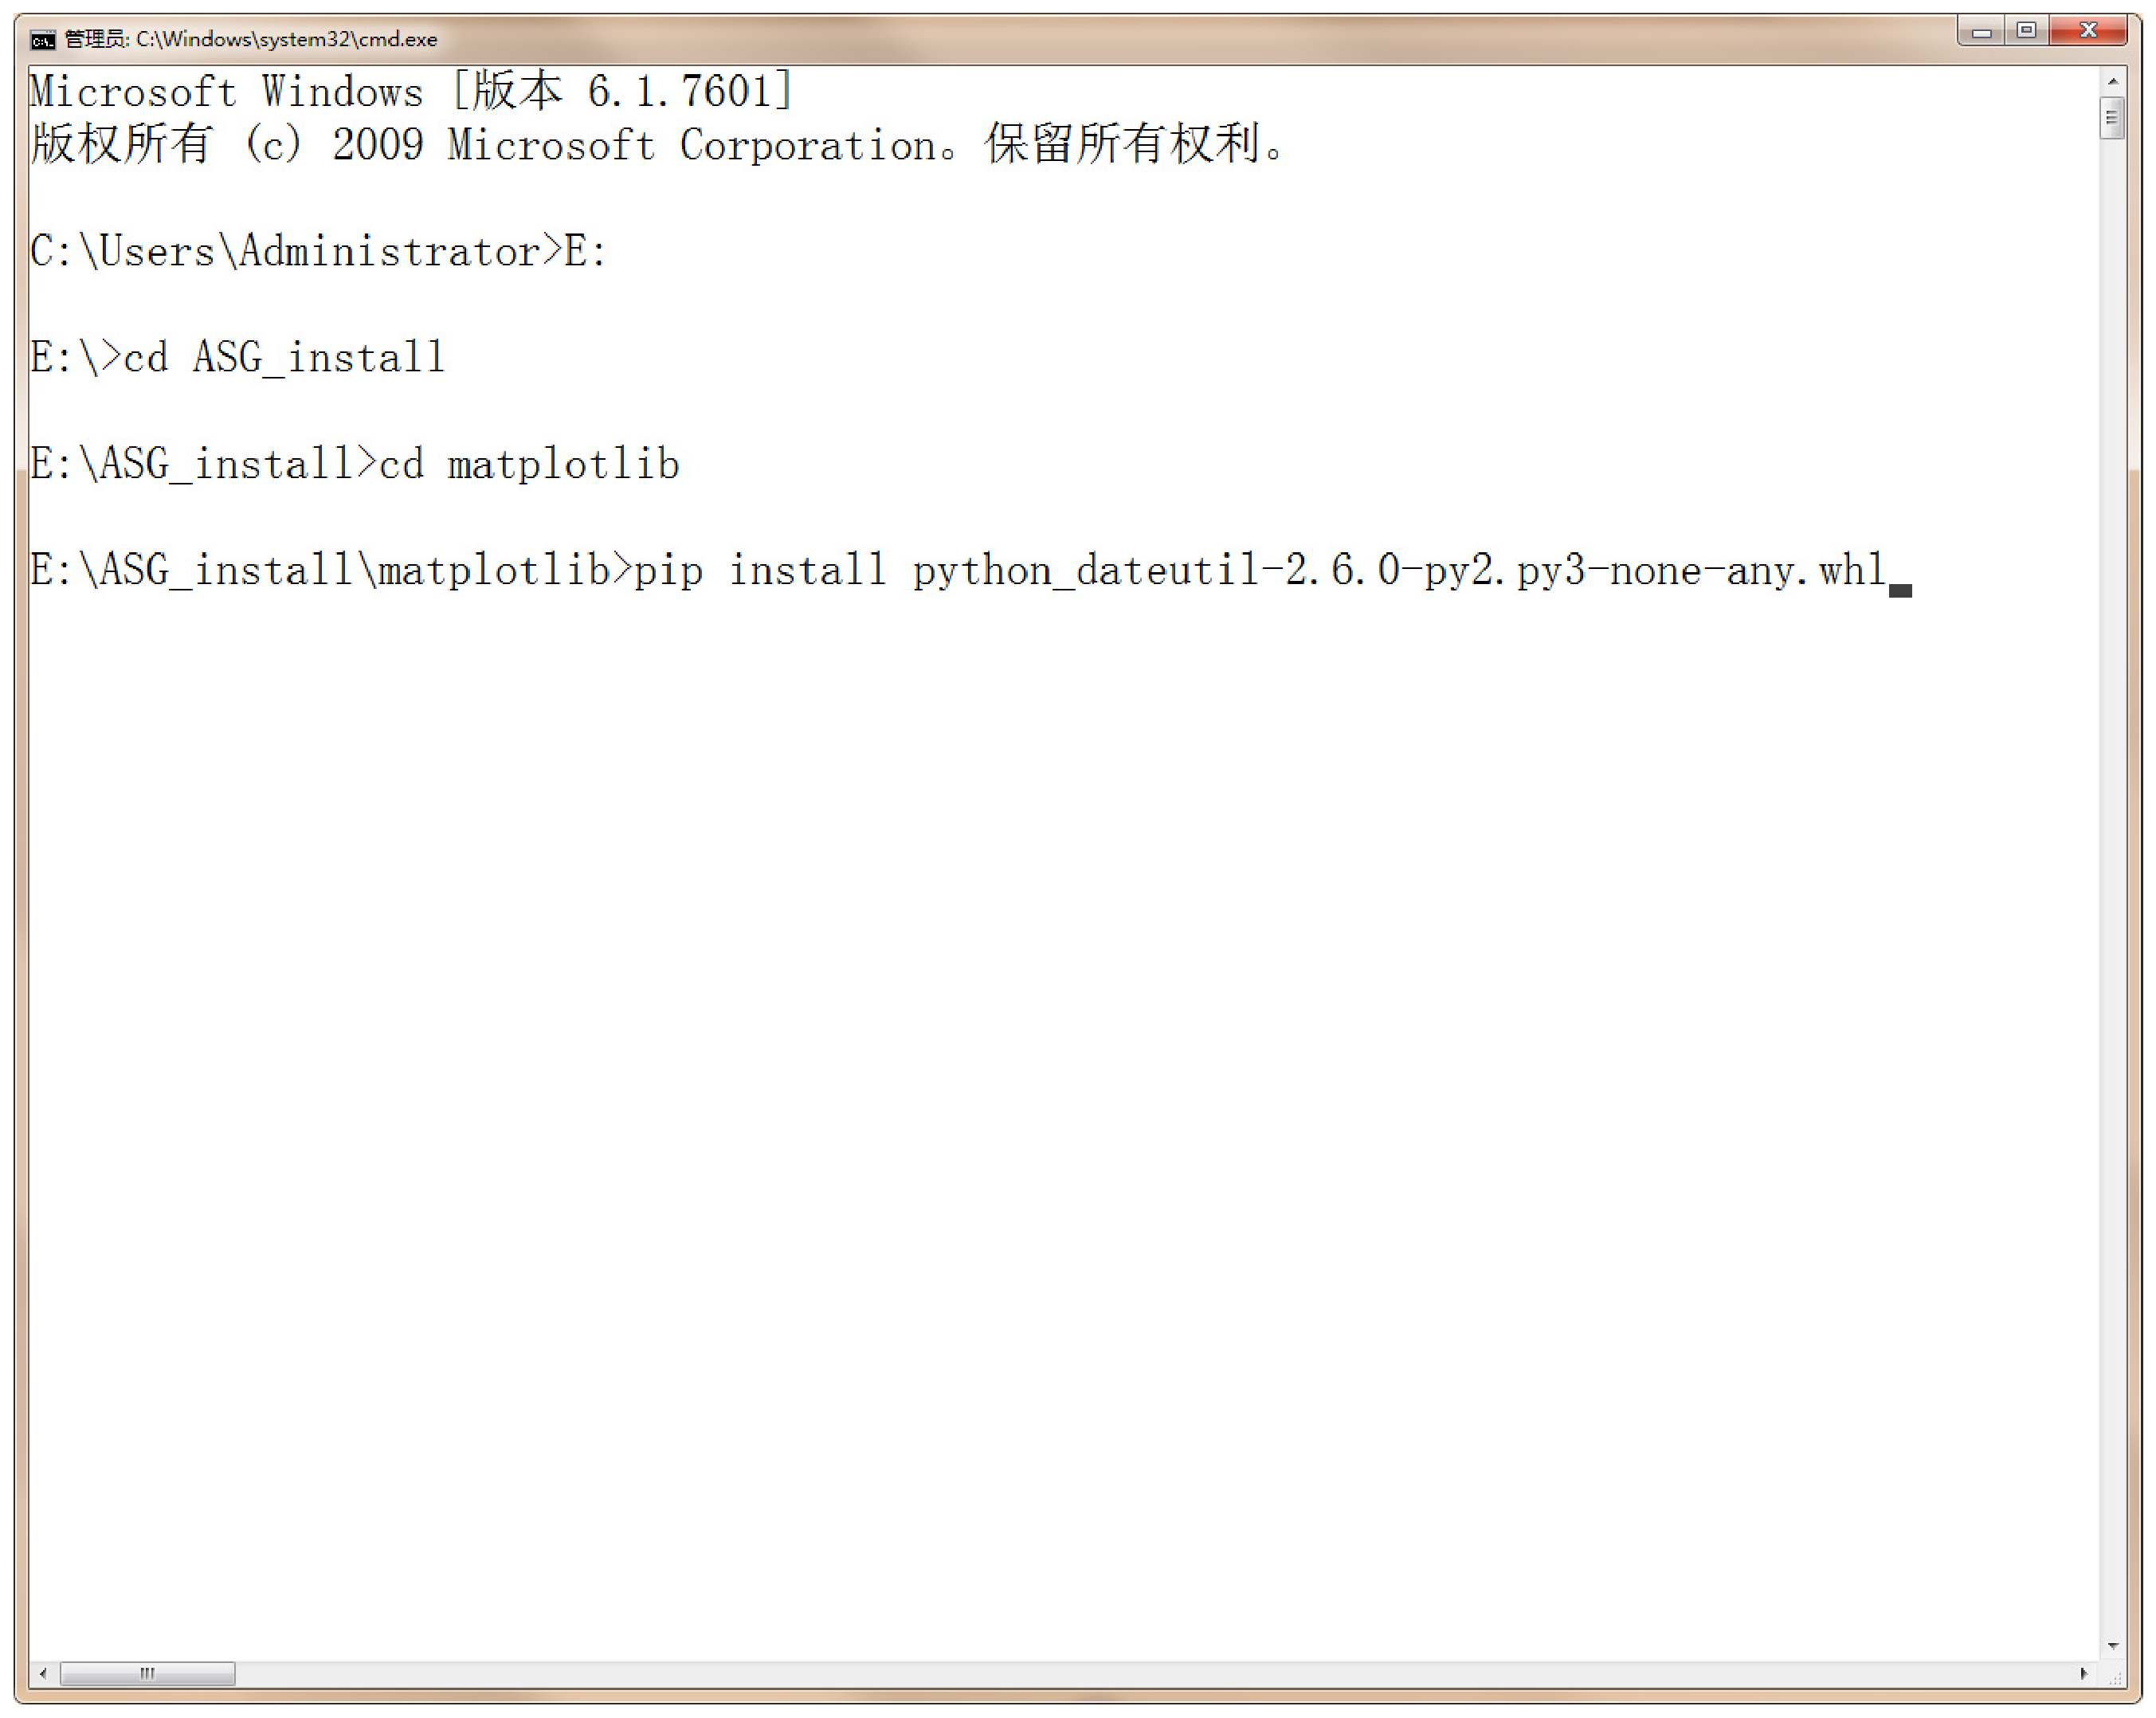
\includegraphics[height=7.5cm]{fig3_2_0}
\caption{Installation steps of dateutil file}
\end{figure}

\newpage
\noindent$\vcenter{\hbox{\huge$\bullet$}}$\quad\fontsize{12pt}{\baselineskip}\textbf{\heiti{Installing pyparsing :}}

As the installation steps of dateutil file, swich the current directory as the lacation that you deposit the the “matplotlib” folder. Then input “pip install pyparsing-2.2.0-py2.py3-none-any.whl” to install pyparsing file. For example, if user put “ASG\_install” folder in the root directory of E disk, the whole installation procedure will be shown in Fig 3.3 .
%同安装dateutil文件一样,在Windows命令窗口将目录切换到我司提供的matplotlib文件夹所在位置,然后通过“pip install pyparsing-2.2.0-py2.py3-none-any.whl”命令安装pyparsing文件。如用户将ASG\_install 文件夹放在E盘的主目录下,完整安装过程如图3.3。

%进入Windows命令行,然后将目录切换到您存放我司提供的“matplotlib”文件夹所在位置。如图3-3输入命令即可安装pyparsing文件。

\begin{figure}[H]
\centering
%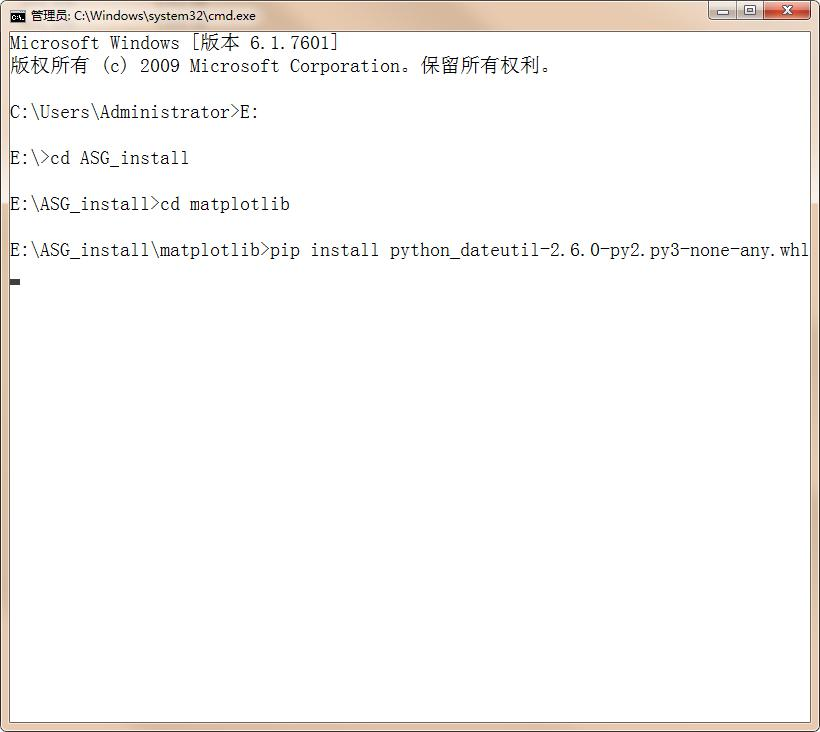
\includegraphics[width=9.6cm,height=7cm]{fig3_3}
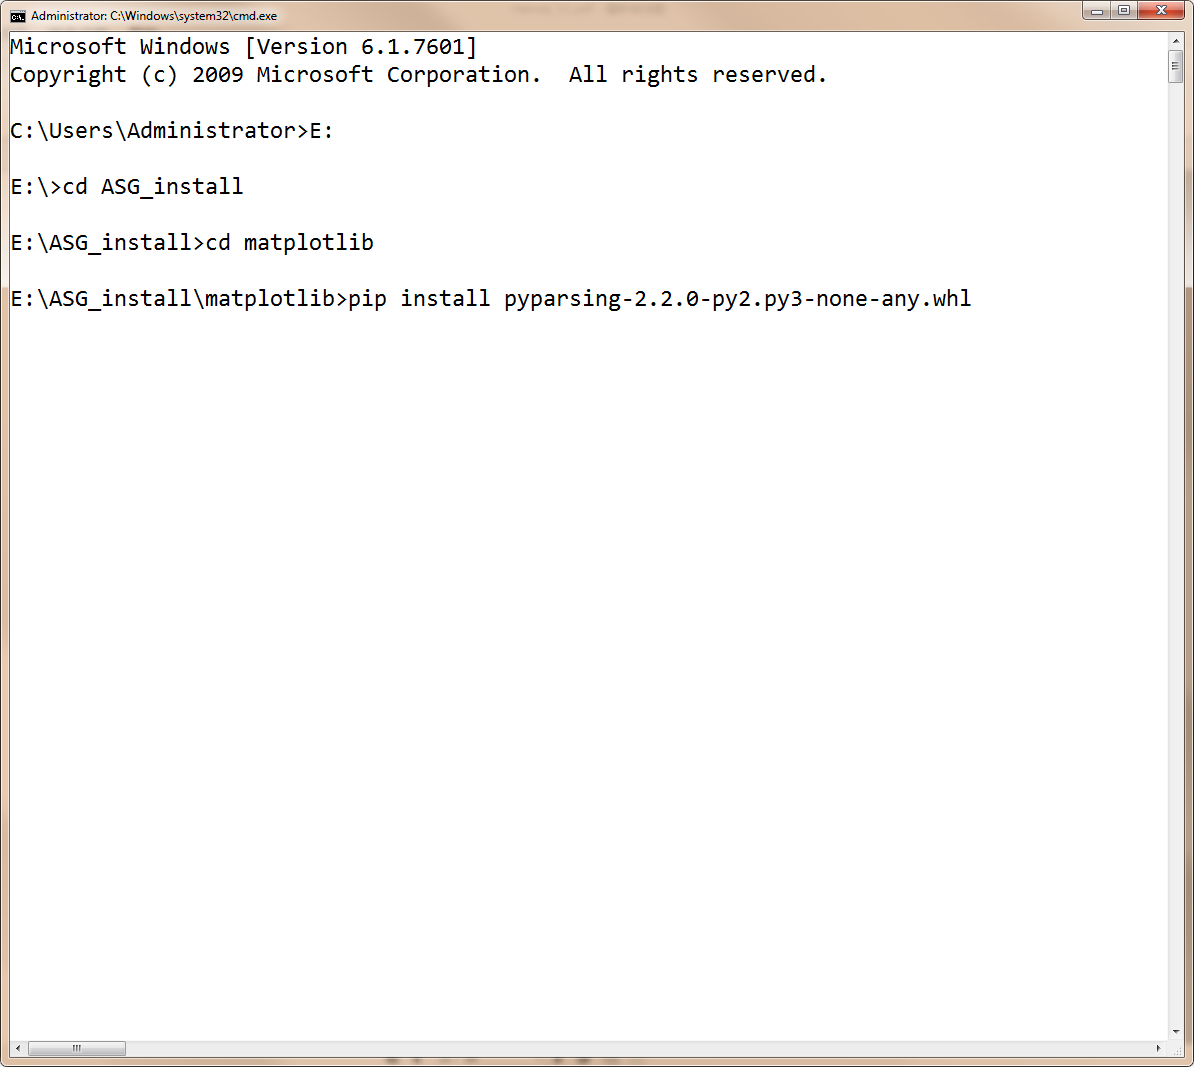
\includegraphics[height=7.2cm]{fig3_3_0}
\caption{Installation steps of pyparsing file}
\end{figure}

\noindent$\vcenter{\hbox{\huge$\bullet$}}$\quad\fontsize{12pt}{\baselineskip}\textbf{\heiti{Installing numpy :}}

Enter the command window and switch the current directory as the location that you deposit the “numpy” folder. Then user input “pip install numpy-1.12.1-cp27-none-win\_amd32.whl” to install the package. For example, if user put “ASG\_install” folder in the root directory of E disk, the whole installation procedure will be shown in fig 3.4 . 
%在Windows命令窗口将目录切换到存放我司提供的numpy文件夹所在位置,然后通过“pip install numpy-1.12.1-cp27-none-win\_amd32.whl”命令安装numpy库。如用户将ASG\_install文件夹放在E盘的主目录下,完整安装过程如图3.4。
\begin{figure}[H]
\centering
%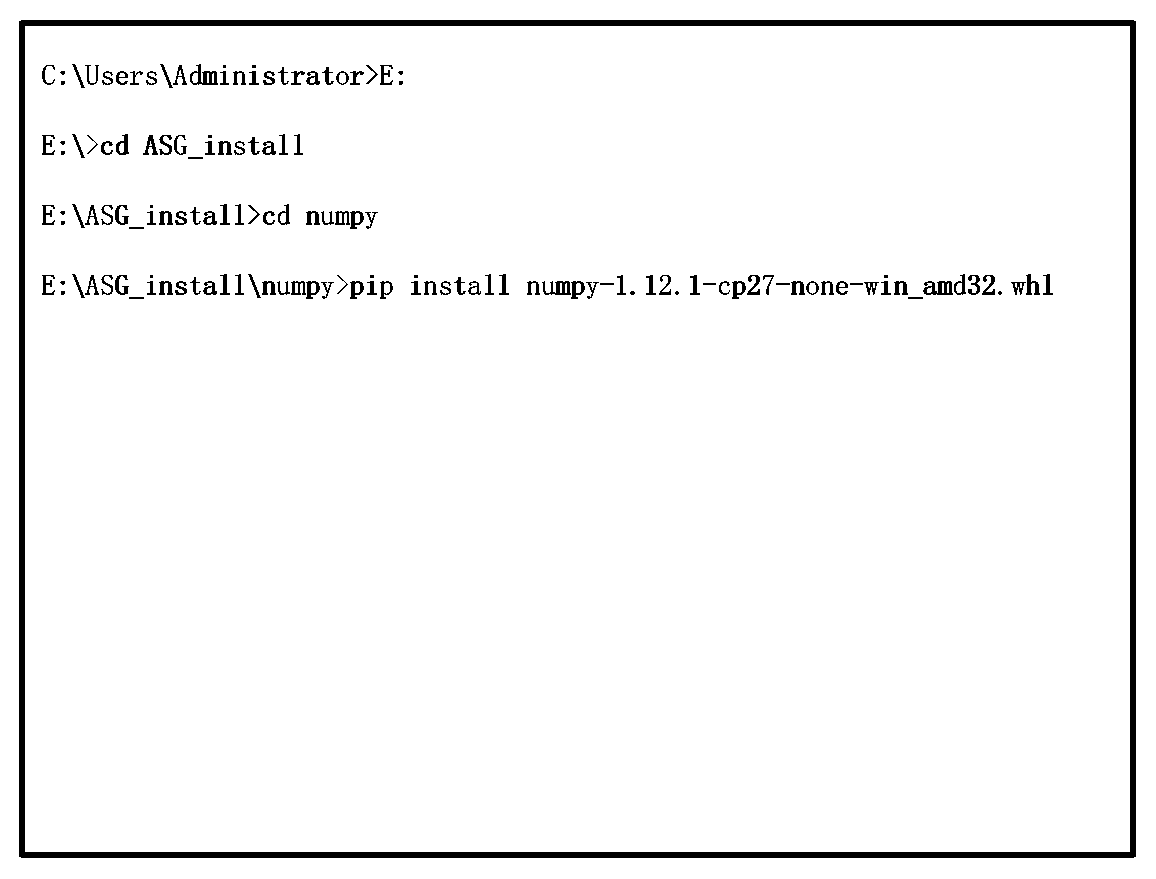
\includegraphics[width=9.6cm,height=7cm]{fig3_4}
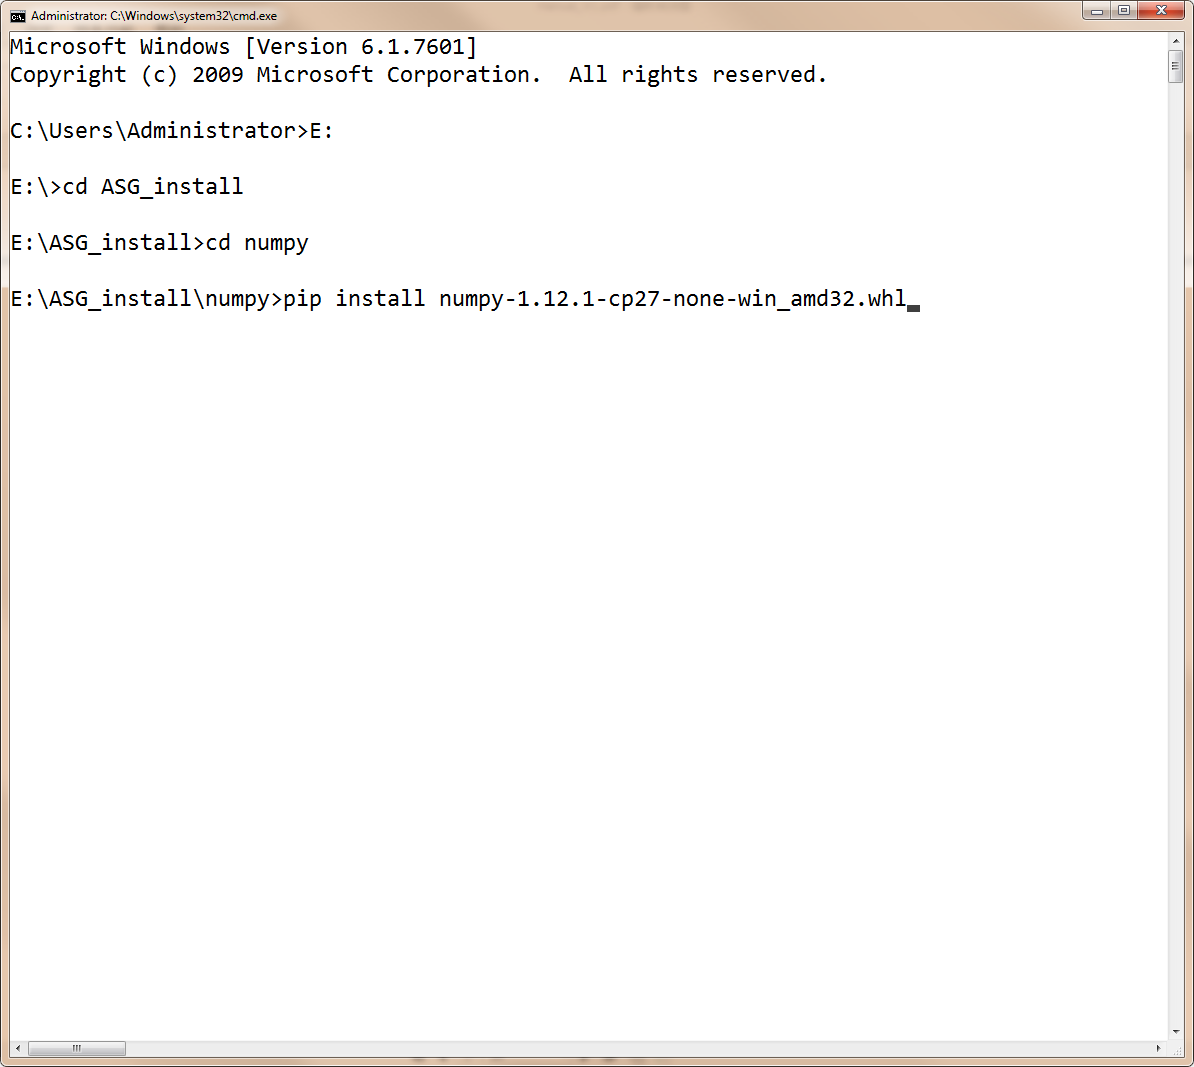
\includegraphics[height=7.2cm]{fig3_4_0}
\caption{Installation steps of numpy}
\end{figure}

\newpage
\noindent$\vcenter{\hbox{\huge$\bullet$}}$\quad\fontsize{12pt}{\baselineskip}\textbf{\heiti{Installing six :}}

Enter the command window and switch the current directory as the location that you deposit the “six” folder. Then user input “pip install six-1.10.0-py2.py3-none-any.whl” to install the package. For example, if user put “ASG\_install” folder in the root directory of E disk, the whole installation procedure will be shown in Fig 3.5 .
%在Windows命令窗口将目录切换到存放我司提供的six文件夹所在位置,然后通过“pip install”命令来安装six库。如用户将ASG\_install 文件夹放在E盘的主目录下,完整安装过程如图3.5。
\begin{figure}[H]
\centering
%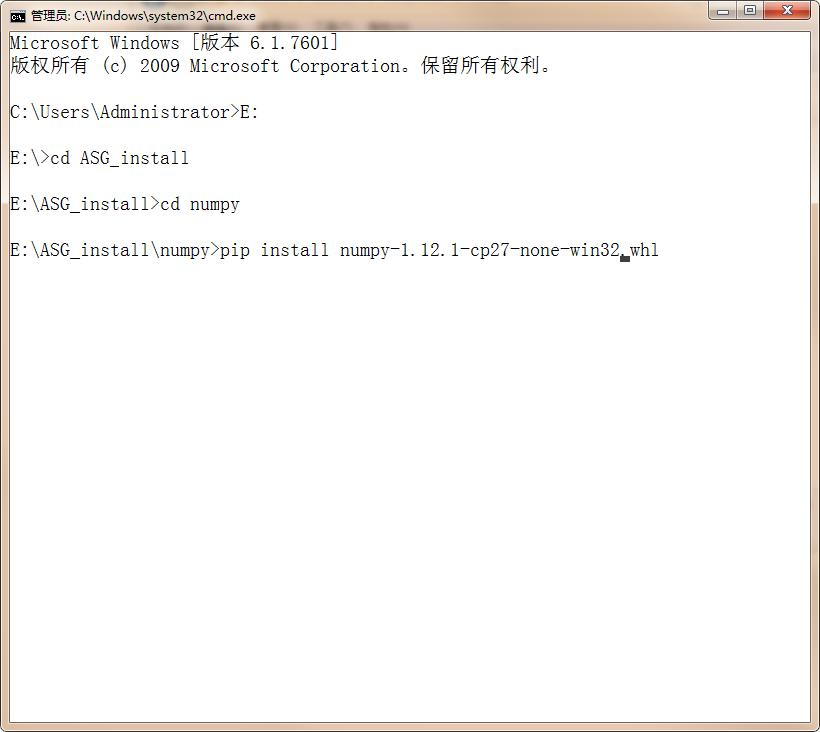
\includegraphics[width=9.6cm,height=7cm]{fig3_5}
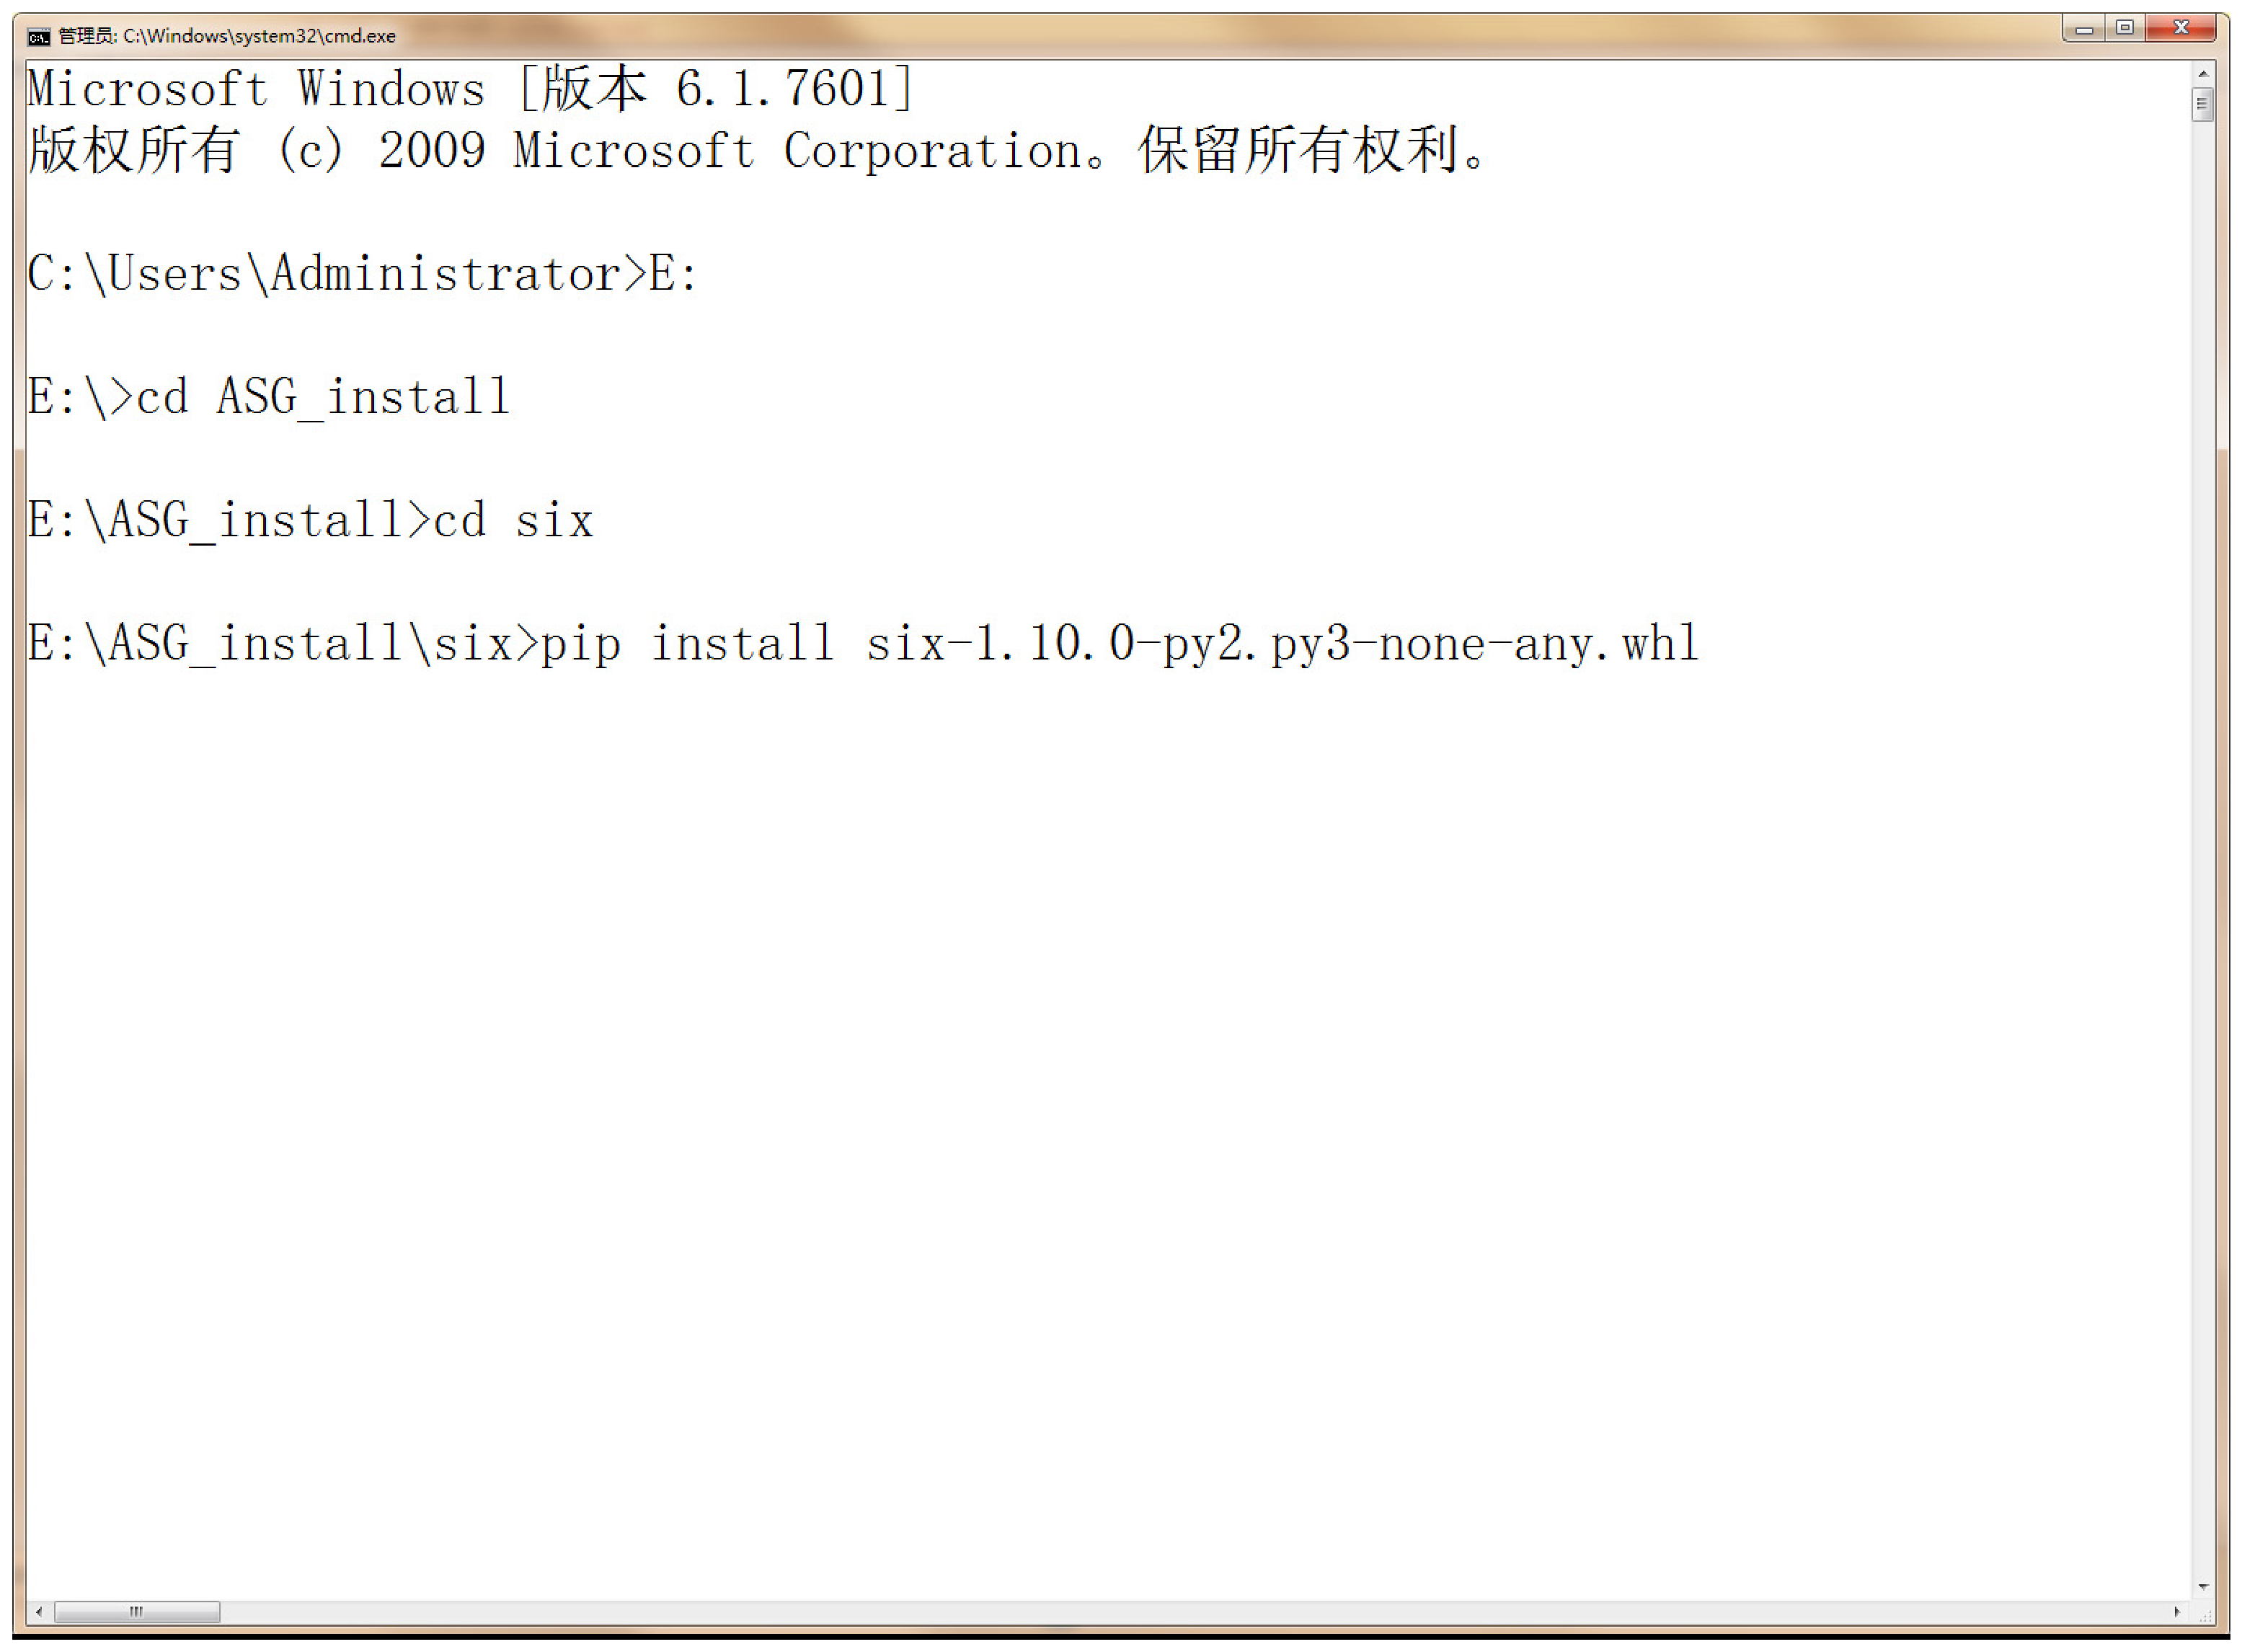
\includegraphics[height=7.5cm]{fig3_5_0}
\caption{Installation steps of six}
\end{figure}

\vspace{0.8cm}
\section{\heiti Installing USB driver}

When a computer connect to the product for the first time, USB driver will be installed automatically. Right click “Computer” → “ ” → “ ”, if you find “EZ-USB FX2 GPIF to Ext FIFO Example using Single Transactions”, you need to install USB driver manually. Please right click “EZ-USB FX2 GPIF to Ext FIFO Example using Single Transactions” → “ ” → “ ”, and then switch current directory as the location that you deposit the “Drivers” folder in “ASG\_install” folder.    
%在一台计算机上首次连接产品时,系统会自动安装产品运行所需的USB驱动程序。请右键“计算机”→“管理”,点击“设备管理器”,查看USB 驱动程序安装是否成功。若在“通用串行总线控制器”找到驱动未安装成功的设备中有“EZ-USB FX2 GPIF to Ext FIFO Example using Single Transactions”一项,则需要手动安装驱动程序(右键选择该设备→ 更新驱动程序软件→浏览计算机以查找驱动程序软件),选择目录至我司为用户提供的“ASG\_install” 文件夹下的“Drivers” 文件夹即可。驱动安装成功后,在设备管理器中可以看到如图3.6 所示的“Cypress FX3 USB StreamerExample Device” 被识别的状态。
\begin{figure}[htbp]
\centering
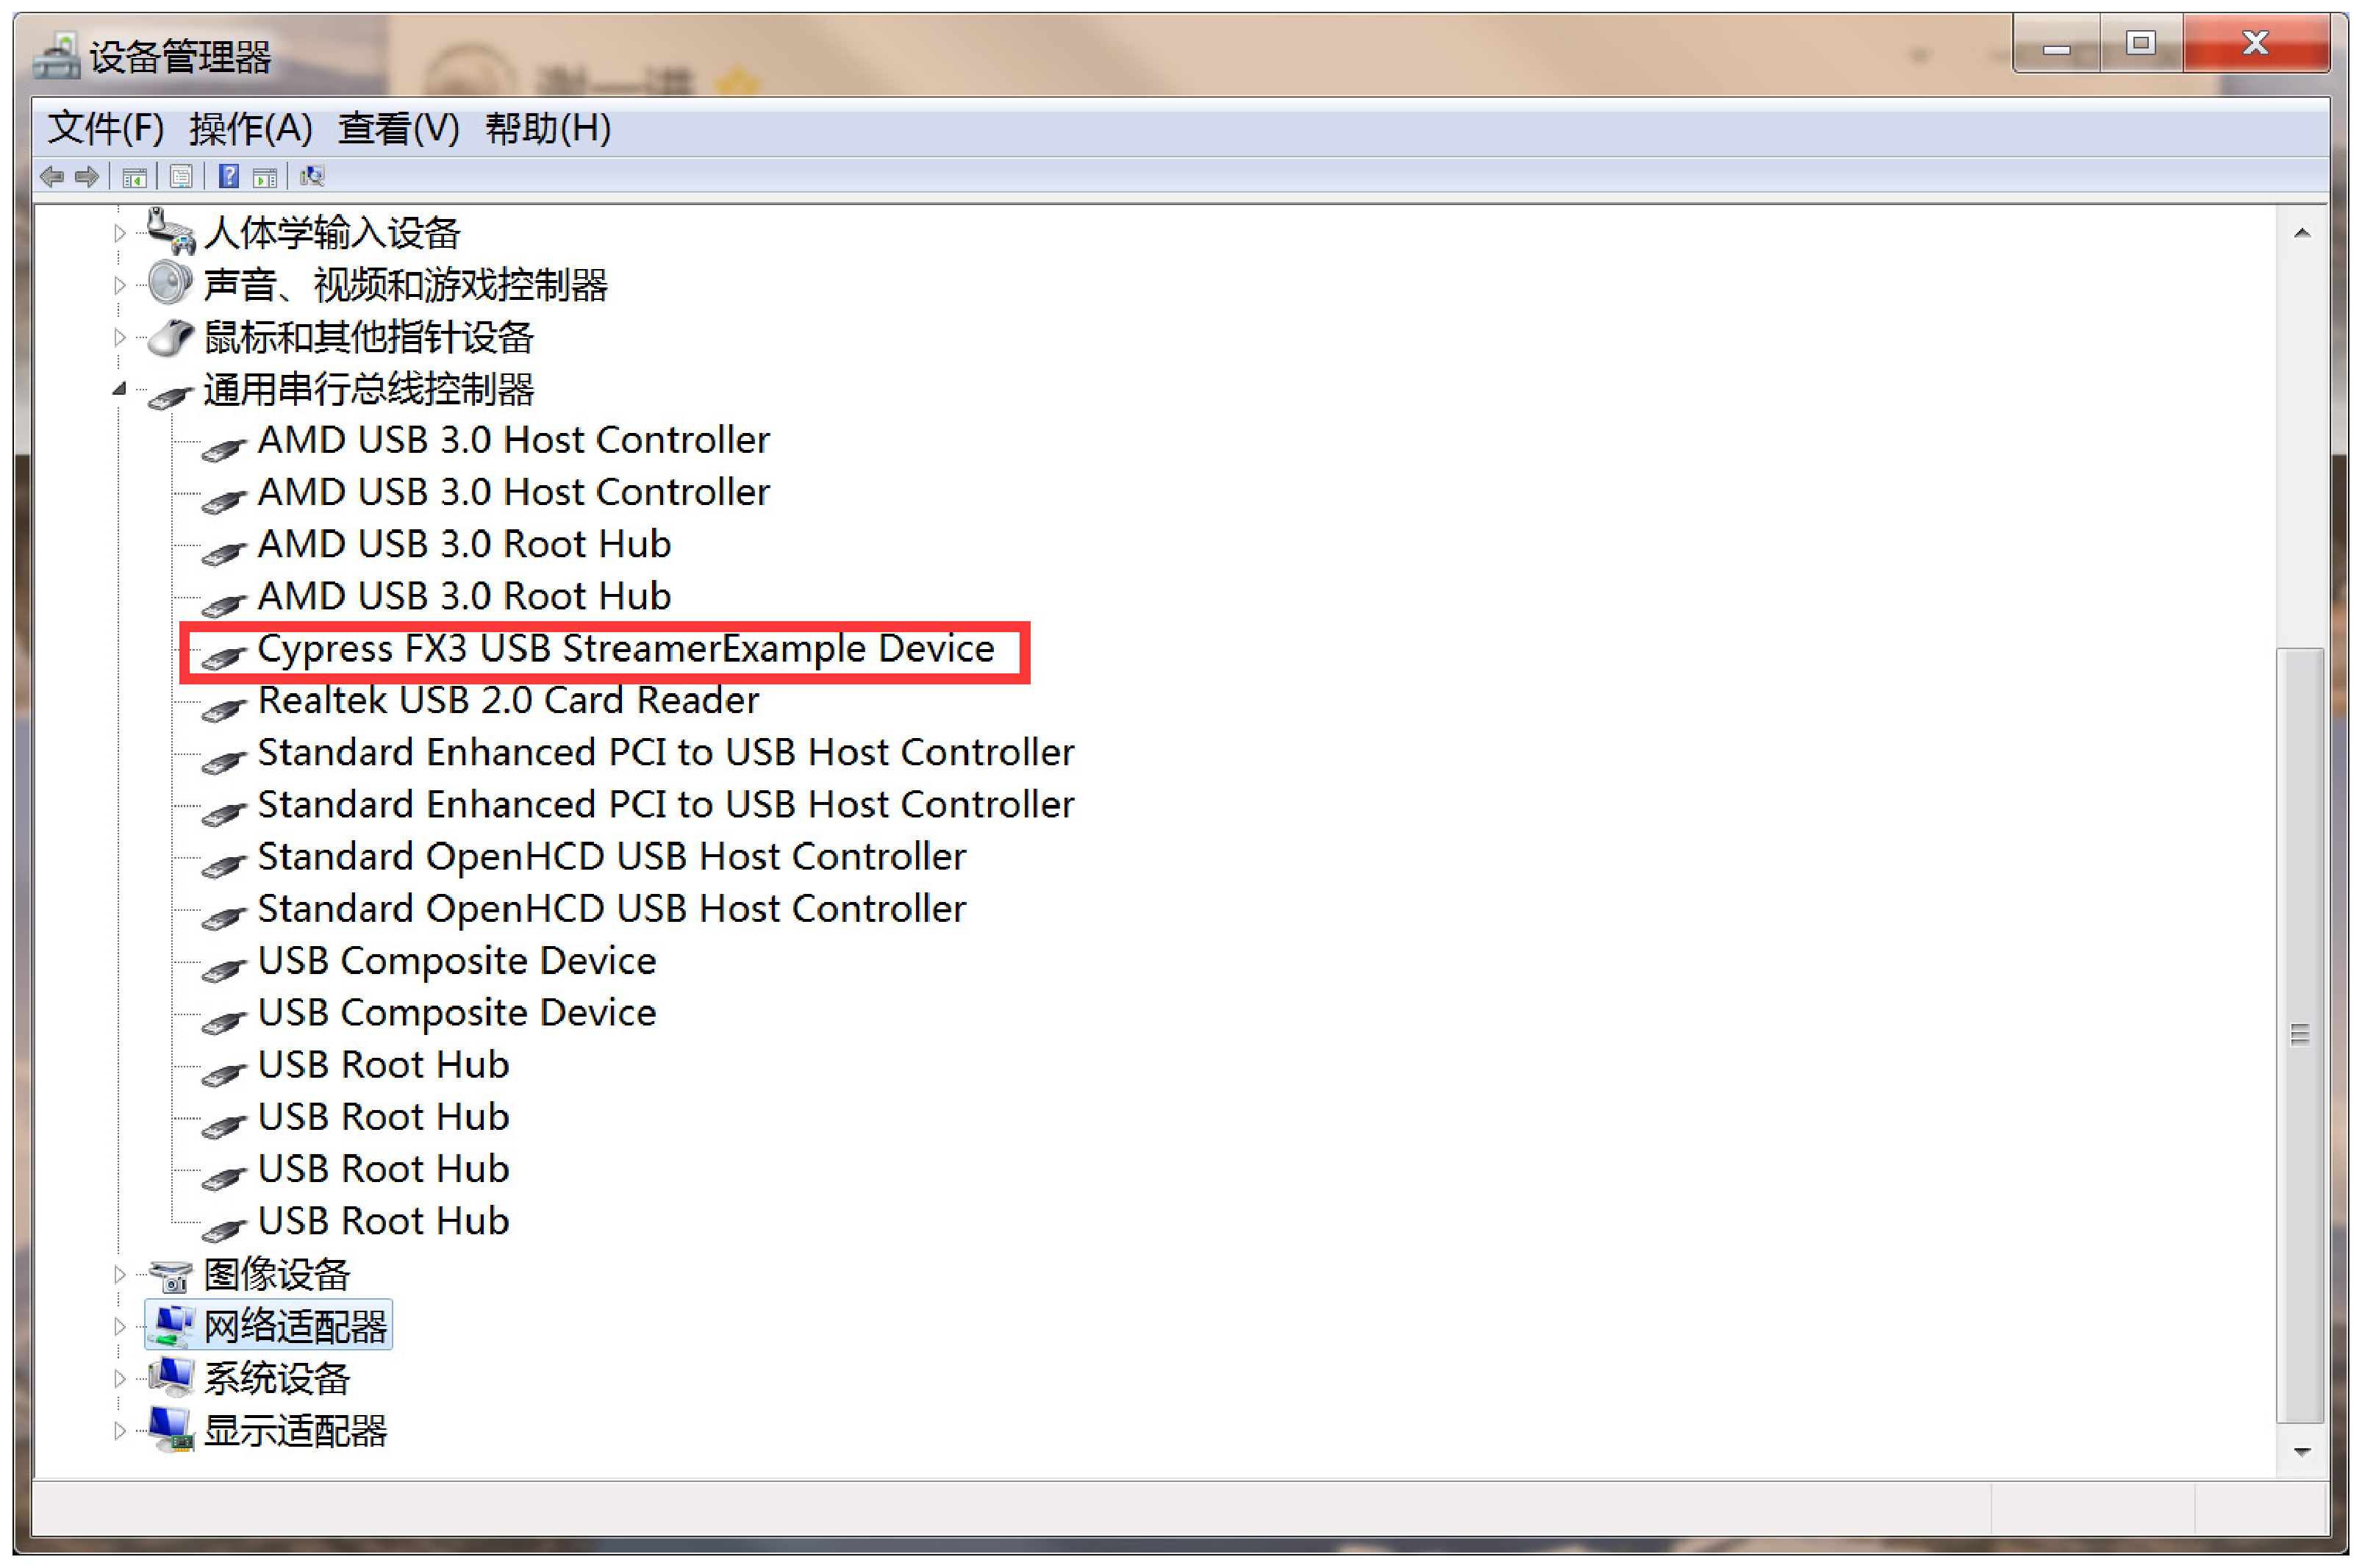
\includegraphics[width=10cm,height= 8.0cm]{fig3_6}
%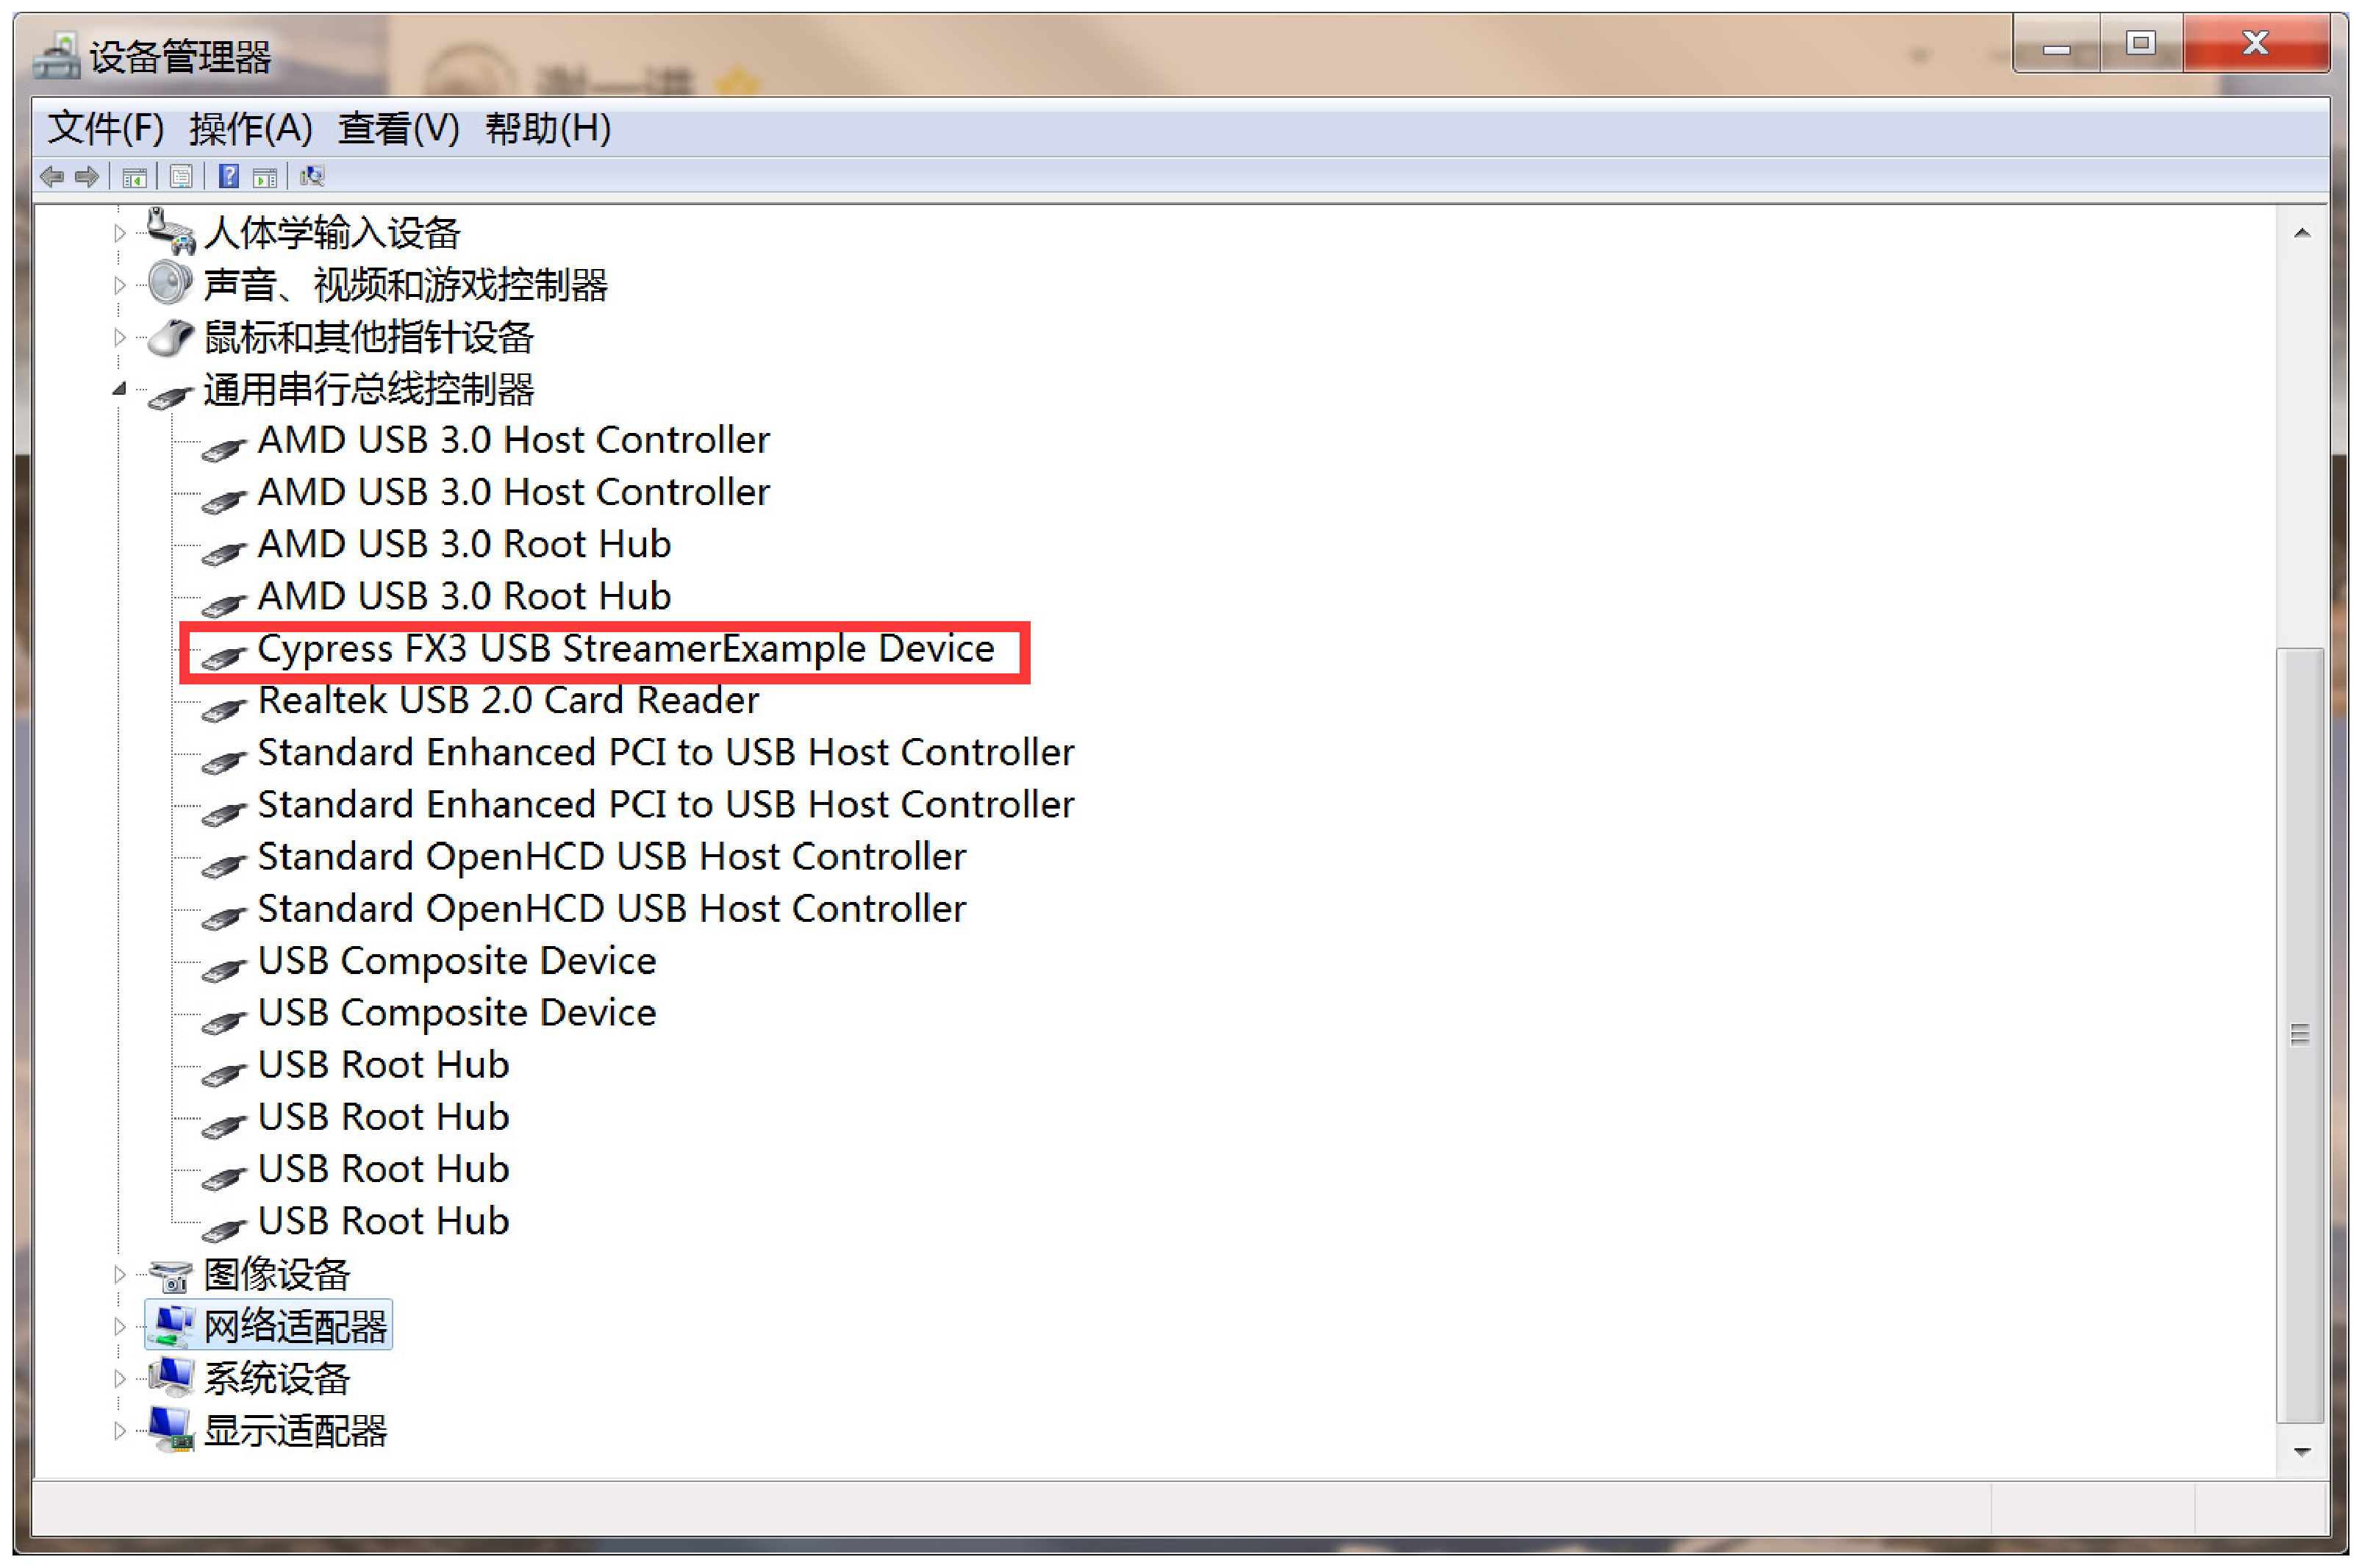
\includegraphics[height= 8.0cm]{fig3_6}
\caption{Installing USB driver}
\end{figure}

When the USB driver has been installed, double click “Cypress FX3 USB StreamerExample Device” to enter the ............. AS Fig 3.7, uncheck 
%驱动程序安装完成后,双击“Cypress FX3 USB StreamerExample Device”打开其属性,进入“电源管理”选项。如图3.7,取消勾选“允许计算机关闭此设备以节约电源”。
\begin{figure}[htbp]
\centering
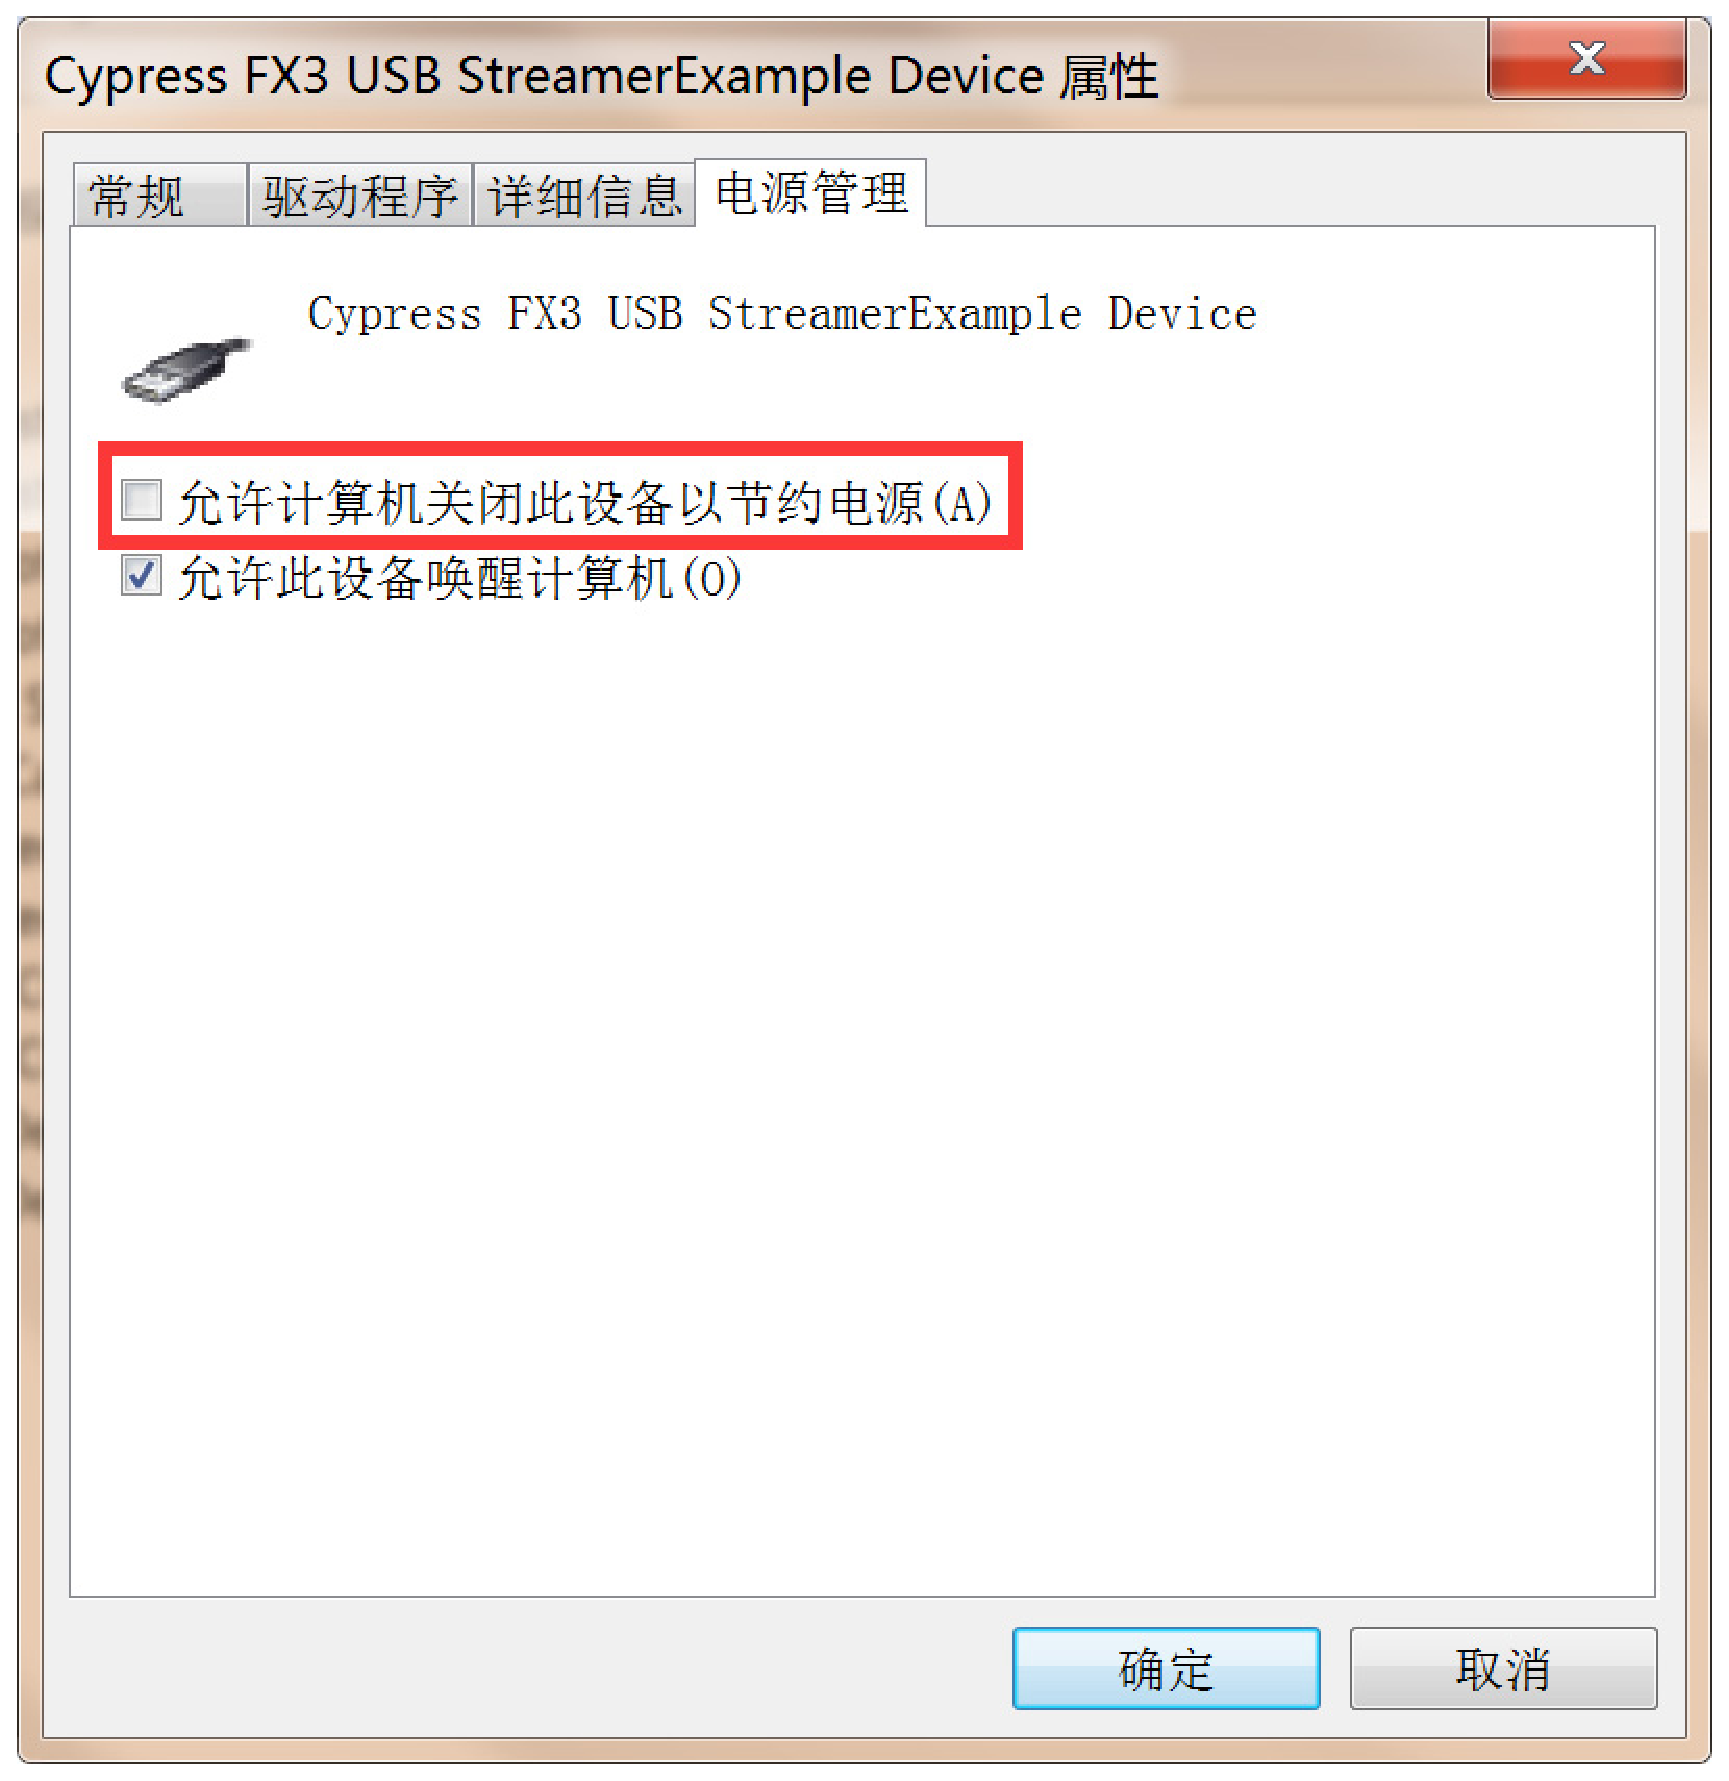
\includegraphics[width=10cm,height=9.0cm]{fig3_7}
%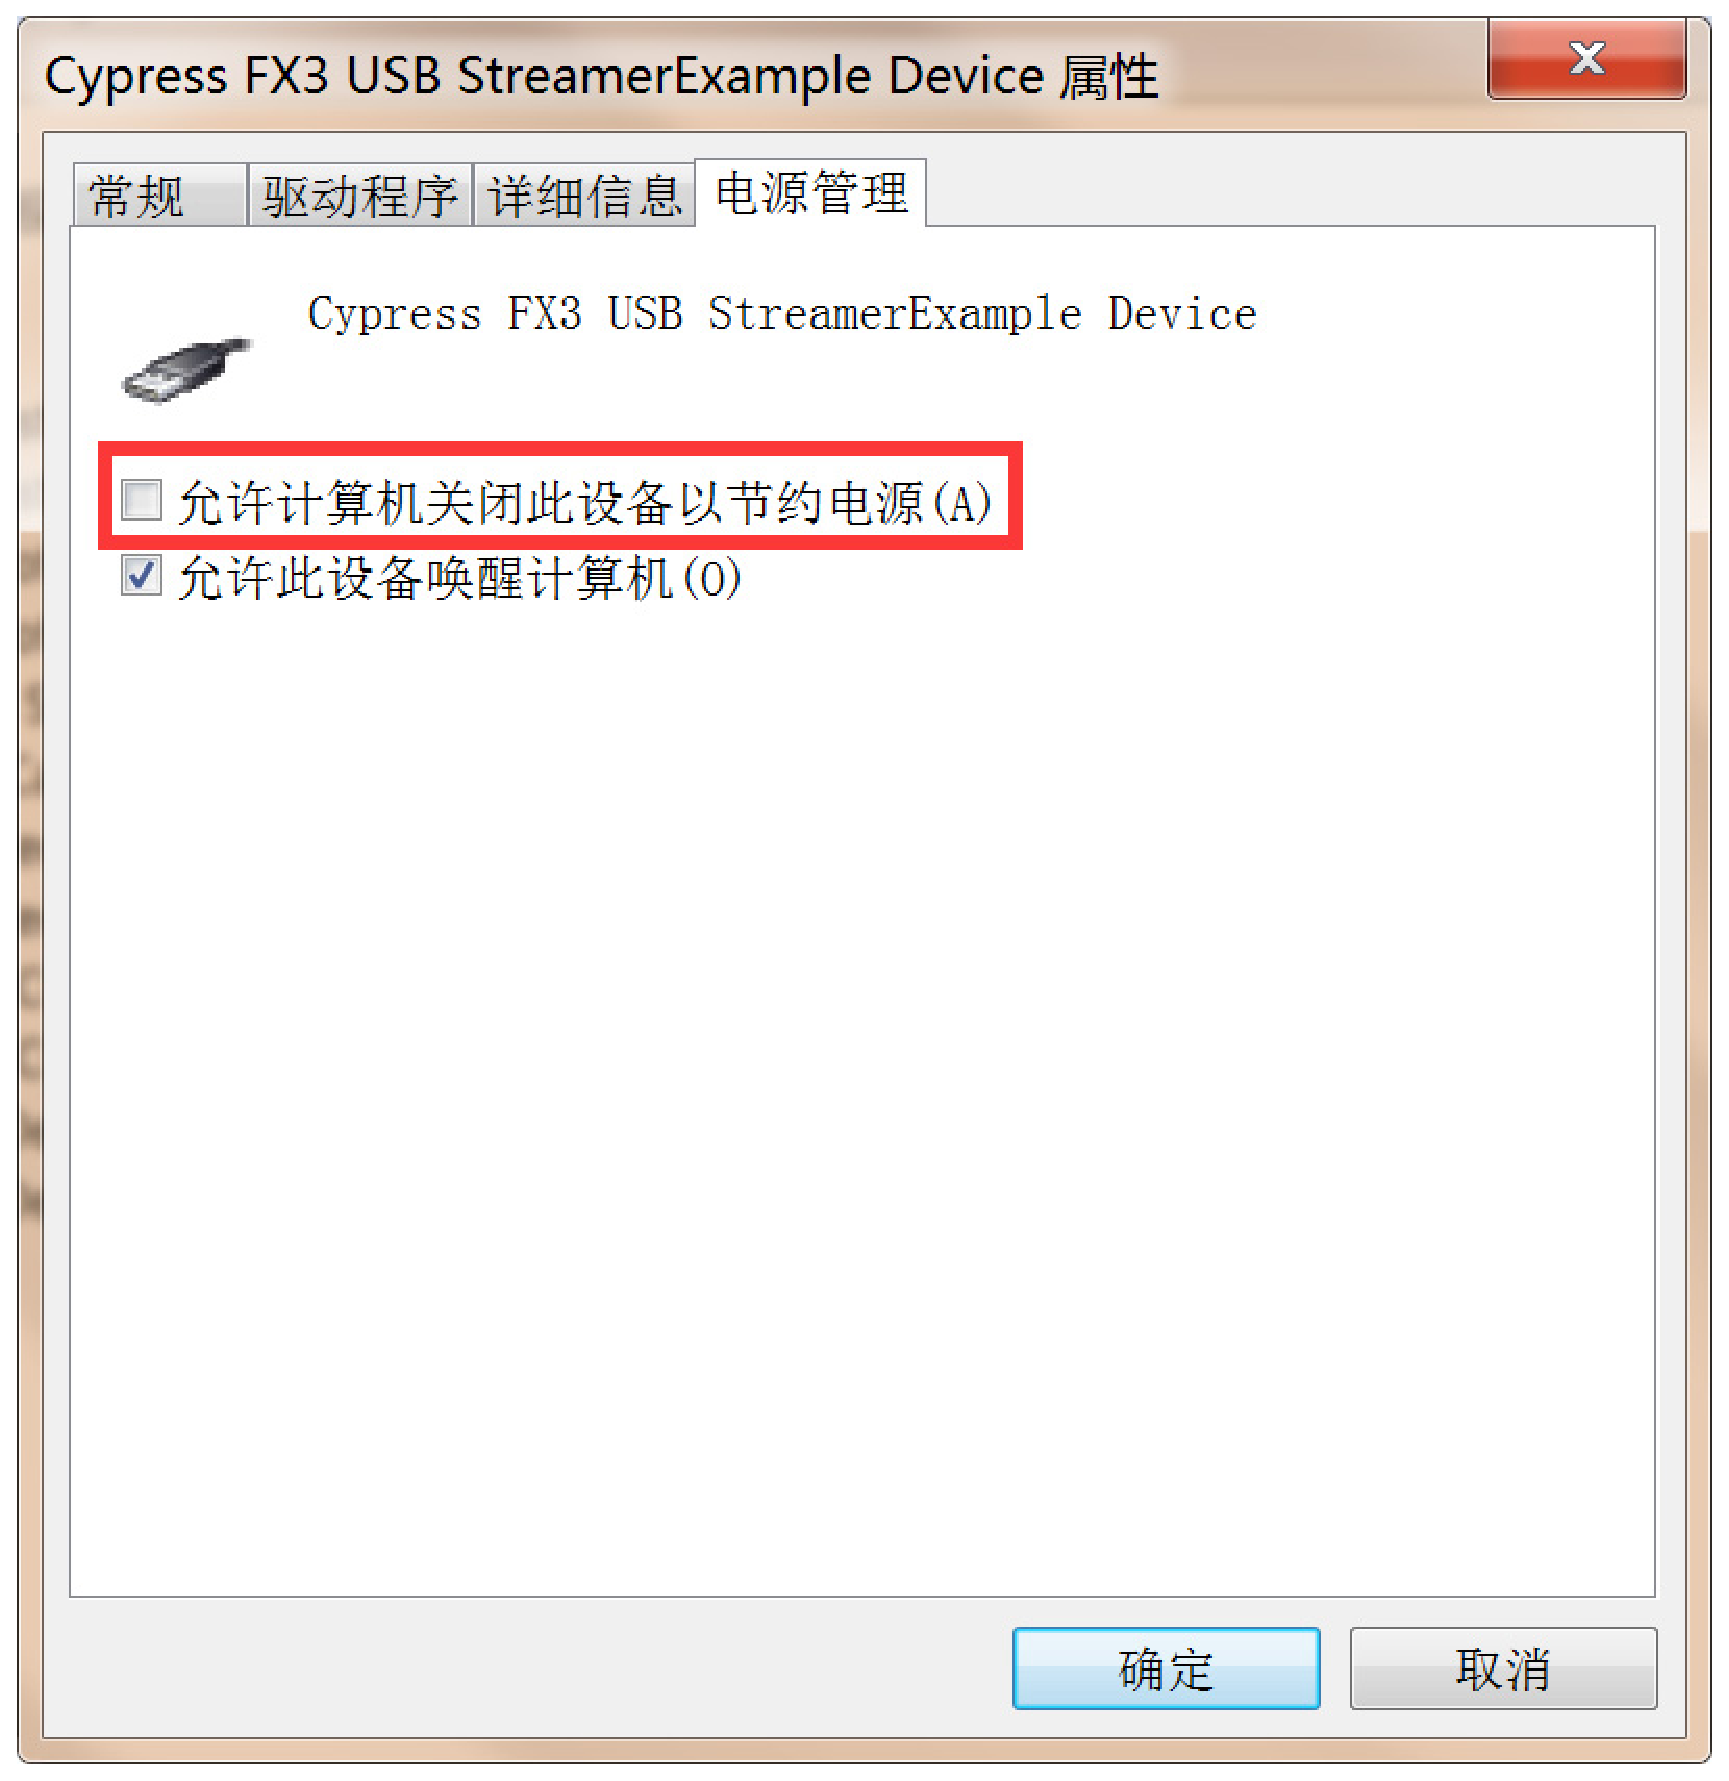
\includegraphics[height=9.0cm]{fig3_7}
\caption{更改电源管理选项}
\end{figure}




